% !Mode:: "TeX:UTF-8"
\documentclass[runningheads,a4paper]{llncs}

\usepackage{amssymb}
\setcounter{tocdepth}{3}
\usepackage{graphicx}
\usepackage{url}

\usepackage{enumitem}
\usepackage[ruled,vlined,linesnumbered]{algorithm2e}
\usepackage{subfigure}
\usepackage{amsmath}%math symbols
\usepackage{bm}
\usepackage{multirow}
\usepackage{comment}


\title{An Efficient Online Event Detection Method for Microblogs via User Modeling \thanks{This research is supported by the Natural Science Foundation of China (Grant No. 61300003, 61572043), and the Specialized Research Fund for the Doctoral Program of Higher Education (Grant No. 20130001120001).}}
% a short form should be given in case it is too long for the running head
\titlerunning{An Efficient Online Event Detection Method for Microblogs}


\begin{document}
\author{Weijing Huang\inst{1} \and Wei Chen\inst{1} \thanks{Corresponding author.}\and Lamei Zhang\inst{2}\and Tengjiao Wang\inst{1}}
\institute{Key Laboratory of High Confidence Software Technologies (Ministry of Education), EECS, Peking University, Beijing, China \and 
Baidu Inc., Beijing, China\\ 
\path{huangwaleking@gmail.com,{pekingchenwei,tjwang}@pku.edu.cn,}\\ 
\path{citlmzhang@163.com}
}
%
\authorrunning{Weijing Huang et al.}
\toctitle{Lecture Notes in Computer Science}
\tocauthor{Weijing Huang et al.}
\maketitle
% BEGIN
% To Proceeding Editors:
% Special codes there for remove page numbers in the LaTeX documents
\thispagestyle{empty}
\pagestyle{empty}
%
% END
%

\begin{abstract}
Detecting events in microblog is important but still challenging. As tweet stream is a mixture of user interests and external events, it's expensive to distinguish them.
Existing methods are ineffective since they ignore user interests or only model interests and events on a fixed dataset without scalability. In this paper, we introduce an online learning model User Modeling Based Interest and Event Topic Model (UMIETM). UMIETM (1) exploits user modeling's information to discover events, which usually capture attentions from users with different interests, and (2) treats the arriving data as stream and run the detection in online learning style. Furthermore, UMIETM can handle dynamic increased vocabulary in tweet stream. The UMIETM is verified on the real dataset which spans one year and contains 16 million tweets, and it outperforms state-of-the-art models in quantitative.
\keywords{event detection, online learning model, microblog stream, user modeling.}
\end{abstract}
\section{Introduction}
Detecting events in microblog is very important as the microblog has become one of the most popular sites for users to publish and get recent news.
However it is still a challenging task, for the reason that tweets are (1) in large scale and (2) in a mixture of user interests and external events.
Users post tweets not only for reporting breaking news, but also talking about interest related affairs.
Existing methods are insufficient in this scenario, such as \cite{lau2012line} which is ineffective when ignoring user interests, and \cite{timeUserLDA2012finding} which lacks scalability when considering user interests but on a fixed dataset.

In another way, user profile or user description is vital in social media. 
And the existing event detection lacks the exploiting of them.
Users describe themselves in profiles to show their interests, locations, occupations or identifications.
These factors are stable and the high generalization of user's characteristics.
One example is Biz Stone\footnote{https://twitter.com/biz} whose profile is \textit{Co-founder of Twitter, Medium, and now Co-founder and CEO of Askjelly.com}. We read his recent 100 tweets, and found 7 tweets talking about Twitter and 36 about Jelly.
This example suggests that user profile is stable to reflect user's interests.
As another example, the profile of a Chinese microblog user @hadoopchina\footnote{http://weibo.com/hadoopchina} is \textit{\#Cloud}, \textit{\#YARN}, \textit{\#Spark}, \textit{\#Big\_Data}, \textit{\#Hadoop}. He mainly tweets IT news until external events happen, such as celebrating spring festival.
This suggests profile can help to distinguish events from user interest-related tweets.
Although some accounts do not have the accurate self-descriptions, they can be augmented by gathering their followings' self-descriptions.
And the user profile information can be utilized to model users' long term interests.

In this paper, we introduce an online learning model, the \textit{User Modeling Based Interest and Event Topic Model} (UMIETM) to discover the bursty events, taking users' profiles into consideration which indicate long term interests.
In UMIETM, the bursty events can be better confirmed when the events receive the attentions from users with different interests.

It's also very interesting when we treat the event detection in microblogs as a kind of crowd sourcing service from different twitterers.
As the old saying "Birds of a feather fly together", there must be something happened when all birds fly. 
We take user profiles as the strong signal to indicate user's behavior or interests.
When different twitterers with different interests post or retweet the same thing, they are telling us that we should pay attention to what they have paid attention to.
We take this intuition into our event detection in microblogs.

The main contributions in our paper can be summarized as follows.
\begin{enumerate}[topsep=0pt,itemsep=-1ex,partopsep=1ex,parsep=1ex]
\item The proposed model UMIETM exploits user modeling's information to discover bursty events, which usually captures attention from users with different interests.
\item The UMIETM is further scaled up to treat the arriving data as stream and run the event detection in online learning style, and is able to handle the dynamic increased vocabulary in tweet stream.
\item We conduct the experiment on the real microblog dataset which spans one year and contains 16 million tweets, and verify that the better user interest modeling can lead to  better performance of event detection.
\end{enumerate}

%The rest paper is organized as follows.In Section 2, the related work about event detection and user modeling is discussed. Section 3 describes the model UMIETM how to exploit the user modeling information in event detection task. Quantitative and qualitative evaluations on real microblog dataset are shown in Section 4. Conclusion and future work are discussed in section 5.

\section{Related Work}
\textbf{Event Detection.} Study of event detection on text stream can be divided into three ways: word frequency based, text similarity based and topic model based.

Several word frequency methods have been developed for event detection such as Discrete Fourier Transform\cite{he2007analyzingDFT}, wavelet analysis \cite{weng2011eventWavelet}.
They treat the word's document frequency along timeline as time series and do the analysis in frequency domain. 
DFT method suffers the problem that it can not locate the time point for bursty.
The complexity of wavelet analysis based method used by EDCoW\cite{weng2011eventWavelet} is very high, so its scalability is limited. 

 Text similarity based online event detection methods\cite{petrovic2010streaming}\cite{mccreadiescalable}  suffer from the lexical variation which means different words describe the same events.
 Similarity based method can successfully detect the tweet which is retweeted by many times, but fails to find out the event which is described from many different perspectives.
 As a result, many events are duplicately detected due to their popularities, which may bury other events and overwhelm users with duplicated unwanted content.


In contrast, topic model can handle the lexical variation problem with word co-occurrence\cite{blei2003latent}.
As many events are highly related to topics, a number of methods based on topic model have been proposed for event detection, including online detection and offline detection.
Lau\cite{lau2012line} introduces an online topic model to track emerging events in microblogs.
It can deal with a massive of tweets, but it doesn't filter out the tweets related to user interests.
Diao\cite{timeUserLDA2012finding}\cite{diao2013unified} show that event detection can benefit from filtering out user interest related tweets. 
And Yan\cite{Yan:2015wm} models the bursty topic by incorporating burstiness of biterms as prior knowledge.
But they are different from ours.
As these models need the whole dataset as the input, they are offline detections, which is not scalability for large dynamic dataset such as microblogs.
Instead, we gather user's self-description and the followings' self-description as user profile which is stable to characterize user interests. 
Based on this fine-grained user modeling information, user's long term interest related tweets and short term bursty event related tweets can be distinguished in online style, and can be efficiently applied on microblogs.

\textbf{User Modeling.} Since user modeling has the significant impact on users' activities on microblogs, the usage of user modeling has drawn attention in many research fields. 
\cite{zhao2013inferring} exploits user modeling information and network topology to infer user's role in social network.
\cite{yoshida2013toward} also introduces user modeling to community detection where some edges are not observable, but user profile can provide additional information.User modeling can be carried out to obtain web users' demographics information \cite{culotta2015predicting} (e.g., gender, age, ethnicity, education, income, etc.).
Compared with demographics information, user interests' modeling can be verified more easily \cite{faralli2015large}. 
Different from the above work, we do not only treat the user modeling result as an additional feature, but also an important representative factor for users, who are the source of information in microblogs.


\section{Method}
\subsection{Problem Formulation}
\textbf{User profile.} User usually describes herself or himself by a piece of short text on microblog platform.
This short text can be a continuous string or an array of hash tags, e.g., "\textit{Co-founder of Twitter, Medium, and now Co-founder and CEO of Askjelly.com}" of Biz Stone or "\textit{\#Cloud}, \textit{\#YARN}" of @hadoopchina.
Though it's easy to estimate Biz Stone's interests by his self-description text, it's not always capable of doing so because some users' are very short.
To overcome this limitation, we define \textbf{user profile} \(\bm{p_u}\) as combining user \(u\)'s self-description text with the texts provided by \(u\)'s followings. 
Taking Biz Stone as an example, he follows 696 accounts, in which there are 60 founders, 27 CEOs, 21 Google related, and 9 medium related accounts, etc. 
This example demonstrates that user profile \(p_u\) can be augmented by gathering the followings' information.

\textbf{User modeling.} 
User modeling is used to capturing user's long term interests. 
For example, Biz Stone's long term interests can be inferred as \textit{Social Media}, \textit{Business}, and \textit{Technology} from his user profile \textit{Medium}, \textit{CEO}, and \textit{Google} respectively.

The notations used in this paper are summarized in Table \ref{symbolsInModel}.
We consider \(u\)'s user timeline as  the triple \(\{uid, \bm{p_u},\bm{w_u}\} \), where \(\bm{p_u}\) represents user \(u\)'s profile and \(\bm{w_u}=\{(tweetid, t_{ud},w_{ud})\}\) means the set of tweets posted by user \(u\).
The element of \(\bm{w_u}\) is a triple of tweet id, time stamp \(t_{ud}\) and tweet content \(\bm{w_{ud}}\).



\textbf{Event.} We define the event in the given time window \(t\) as the set of tweets denoted by \( \{ \bm{w_{te}}\}\).
The event related tweets in set \( \{ \bm{w_{te}}\}\)  hold two properties: (1) they are posted by users with different interests (2) they are similar within the set.
The task of event detection is to find out all the events in corpus.
Different methods treat the above properties in different ways: LSH based methods\cite{petrovic2010streaming} treat the difference and similarity in word vector space; while the topic model based methods\cite{timeUserLDA2012finding} take the semantic meaning into consideration.
Under the framework of topic model, we divide the topics into user interest related topics and bursty event related topics, and further promote an online learning model UMIETM.

\subsection{Model Descriptions}
\label{subsec:model}
UMIETM is motivated by two observations: (I)user profiles are more stable to reflect users' interests than tweets; and (II)external events draw global attention in short time.
\begin{figure}
    \includegraphics[width=1.0\textwidth]{img/model.pdf}
    \caption{Illustration of UMIETM (left), and an example user Biz Stone's tweets about his long term interests and  bursty event (SXSW is a music, film and interactive conference and festival hosted on March 11-20) (right).} 
    \label{fig:modelUMIETM}
\end{figure}

To capture Observation I, we enhance the association between profile topic and tweet topic which is inspired by \cite{blei2003modeling}. 
More particularly, the model generates observed data for user \(u\) in two phases as shown in Figure \ref{fig:modelUMIETM}. 
The first phase generates the hidden topic \(s_{un}\) from user interest topic distribution \(\theta_{u}\), then generates profile token \(p_{un}\). 
When \(y_{ud}\) = 0, the second phase generates tweet topic \(z_{ud}\) from associated profile topics \(\{s_{u1},..., s_{un}\}\) uniformly. 
To overcome the deficiency of user profile words, we add the smoothing factor \(\kappa\) for each topic to \(s_{un}\). 
The second phase makes a closer correlation between profile topics and tweet topics. 

For Observation II, we introduce time dependent event distribution \(\eta_t\) and switcher \(y_{ud}\) to distinguish user’s long term interests from short term responses to external events. 
Only if switcher \(y_{ud}\) = 1, tweet topic \(z_{ud}\) will be sampled from multinomial event distribution \(\eta_{t}\).

We introduce UMIETM's generative process and leave the detail of online learning to section \ref{subsec:online}.
We assume that there are \(K\) latent topics corresponding to all users' interests in corpus.
\(\psi_k\) and \(\phi_k\) are profile word distribution and tweet word distribution on \(k\)-th interest topic respectively.
We also assume a background word distribution \(\phi_0\) to filter out common words.
We set \(E\) events as word distributions \(\{\varphi_{te}\}\) in each time window \(t\).


\begin{table}
\centering
\caption{UMIETM's Notations and Generative Process}
\subtable[Notations]{
\scalebox{0.7}{
\begin{tabular}{|l|p{8.5cm}|} \hline
\(T\) & number of time windows     \\ \hline
\(E\) & number of event-related topics in each time window \\ \hline
\(K\) & number of interest-related topics \\ \hline
\(U\) & number of users \\ \hline
\(P_u\) & number of tokens appeared in user \(u\)'s profile \\ \hline
\(D_u\) & number of tweets published by user \(u\) \\ \hline
 \(\alpha\), \(\beta\) & priors of Dirichlet distributions     \\ \hline
 \(\theta_u\) & K dimension vector indicating user \(u\)'s interest distribution \\ \hline
\(p_{un}\) & user \(u\)'s n-th profile token \\ \hline
\(s_{un}\) & the hidden topic of user \(u\)'s n-th profile token \\ \hline
\(\psi_k\) & the user profile token's distribution on k-th profile topic \\ \hline
\(\eta_t\) & the events' distribution in time window \(t\) \\ \hline
\(\pi_u\) & the preference of user \(u\) to participate the discussion of global events \\ \hline
\(y_{ud}\) & the type of user \(u\)'s d-th tweet (\(y_{ud}=0\) indicates interest-related, \(y_{ud}=1\) event-related) \\ \hline
\(t_{ud}\) & the discrete value between 1 and T indicating the timestamp of user \(u\)'s d-th tweet \\ \hline
\(z_{ud}\) & the topic of user \(u\)'s d-th tweet , \(z_{ud} \in \{1,...K\}\) if \(y_{ud}=0\); \(z_{ud}\in\{1,...,E\}\) if \(y_{ud}=1\) \\ \hline
\(\phi_k\) & tweet token's distribution on \(k\)-th interest-related topic \\ \hline
\(\phi_{te}\) & tweet token's distribution on \(e\)-th event-related topic in time window \(t\)\\ \hline
\(x_{udn}\) & the boolean indicator of \(n\)-th token in user \(u\)'s \(d\)-th tweet: background word if \(x_{udn}=0\); non-background word if \(x_{udn}=1\)\\ \hline
\(w_{udn}\) & the n-th token in user \(u\)'s \(d\)-th tweet: may chosen from \(\phi_0\), \(\phi_k\) or \(\phi_{te}\) \\ \hline
\(\rho\) & the Bernoulli parameter for boolean indicator \(x_{udn}\)\\ \hline
\(\phi_0\) & tweet token's distribution on background topic \\ \hline
\(\gamma\), \(\lambda\) & the priors for Bernoulli distributions \\ \hline
\end{tabular}
}
\label{symbolsInModel}
}
\quad
\subtable[Generative Process]{
\scalebox{0.7}{
\begin{tabular}{|l}
\(\rho \sim Beta(\lambda)\), \(\phi_0 \sim Dir(\beta)\) \\
for \(k\)=1 to \(K\): \\
\ \ \(\psi_k \sim Dir(\beta)\), \(\phi_k \sim Dir(\beta)\) \\
for \(t\)=1 to number of time windows: \\
\ \ \(\eta_t \sim Dir(\alpha)\) \\
\ \ for \(e\)=1 to \(E\): \\
\ \ \ \  \(\varphi_{te} \sim Dir(\beta)\) \\
for each user \(u\): \\
\ \ \(\pi_u \sim Beta(\gamma)\) \\
\ \ user interest \(\theta_u \sim Dir(\alpha)\) \\
\ \ for \(n\)=1 to number of \(u\)'s profile tokens: \\
\ \ \ \ \(s_{un} \sim Multinomial(\theta_u)\) \\
\ \ \ \ \(p_{un} \sim Multinomial(\psi_{s_{un}})\) \\
\ \ for tweet \(d\)=1 to \(D_u\): \\
\ \ \ \ \(y_{ud} \sim Multinomial(\pi_u) \) \\
\ \ \ \ if \(y_{ud}\)=0: \\
\ \ \ \ \ \ \(z_{ud} \sim Uniform(\{s_{u1},...,s_{un}\}) \) \\
\ \ \ \ else: \\
\ \ \ \ \ \ \(z_{ud} \sim Multinomial(\eta_{t_{ud}}) \) \\
\ \ \ \ for \(n\)=1 to \(N_{ud}\): \\
\ \ \ \ \ \ \(x_{udn} \sim Bernoulli(\rho)\) \\
\ \ \ \ \ \ if \(x_{udn}\)=0: \\
\ \ \ \ \ \ \ \ \(w_{udn} \sim Multinomial(\phi_0)\) \\
\ \ \ \ \ \ else: \\
\ \ \ \ \ \ \ \ if \(y_{ud}\)=0: \\
\ \ \ \ \ \ \ \ \ \ \(w_{udn} \sim Multinomial(\phi_{z_{ud}}) \) \\
\ \ \ \ \ \ \ \ else: \\
\ \ \ \ \ \ \ \ \ \ \(w_{udn} \sim Multinomial(\phi_{t_{ud},z_{ud}}) \) \\
\end{tabular}
}
\label{tab:GenerativeProcess}
}
\end{table}
Overall, the generative process of user profiles and tweets in UMIETM can be described as Table \ref{tab:GenerativeProcess}.

We also propose the variant IETM to check the significance of user profile.
Different from UMIETM, IETM models user interest related tweets directly. 
If user profile is very important to distinguish user interests from events, UMIETM will outperform IETM, vice versa.

\subsection{Model Inference}
We run collapsed Gibbs sampling to obtain samples of hidden variables.
For space limit, we omit the detail of inference and only list the conditional distribution of each hidden variable.
As there is a coupling between profile topics and tweet topics, the Gibbs sampling should be divided into two phases, first for profiles, second for tweets.

In first inference phase (shown in Algorithm 1 line 2 to line 6) we sample user profile's hidden topic \(s_{un}\) as standard LDA's collapsed Gibbs sampling\cite{griffiths2004finding}, where \(c^{(p)}_{uk}\) is the number of user \(u\)'s profile words assigned to topic \(k\), \(c^{(p)}_{u,.}\) is the total number of profile words of \(u\) and \(c^{(p)}_{kv}\) is the times of profile word \(v\) assigned to topic \(k\).
\begin{scriptsize}
\begin{equation}
\label{timeUserTagLDAIVsamplingForS}
\begin{aligned}
&p(s_{un}=k|s_{\neg{un}},\vec{p},\alpha,\beta)
\propto \frac{c^{(p)}_{uk}+\alpha}{c^{(p)}_{u,.}+K\alpha}
\frac{c^{(p)}_{kv}+\beta}{c^{(p)}_{k,.}+V\beta}
\end{aligned}
\end{equation}
\end{scriptsize}


After the convergence of the first Gibbs sampling phase, we start the second (shown in Algorithm 1 line 7 to line 21).
We joint sample for \(y_{ud}\) and \(z_{ud}\) using Equation(\ref{timeUserTagLDAIVJointSamplingForY0Z}) and (\ref{timeUserTagLDAIVJointSamplingForY1Z}) where \(c^{(0)}_{kv}\) is the number of tweet word \(v\) assigned to \(k\)-th interest topic, and \(n^{(0)}_{kv}\) is the number of word \(v\) in \(d\)-th tweet assigned to \(k\)-th interest topic.
\(c_u^{0}\) and \(c_u^{1}\) denote the number of user \(u\)'s tweets labeled as interest related and event related respectively.
In order to avoid the deficiency of user profile tokens, we add smoothing parameter \(\kappa\) to \(c^{(p)}_{uk}\) in Equation (\ref{timeUserTagLDAIVJointSamplingForY0Z}).

\begin{scriptsize}
\begin{equation}
\label{timeUserTagLDAIVJointSamplingForY0Z}
\begin{aligned}
&p(y_{ud}=0,z_{ud}=k|\vec{y}_{\neg{ud}},\vec{z}_{\neg{ud}},\vec{t},\vec{w},\vec{s},\alpha,\beta,\gamma)\\
&\propto \frac{c_u^{0}+\gamma}{c_u^{1}+c_u^{0}+2\gamma}\frac{c^{(p)}_{uk}+\kappa}{c^{(p)}_{u,.}+K\kappa}
        \frac{\prod_{v=1}^{V}\prod_{b=0}^{n^{(0)}_{kv}-1}{(c^{(0)}_{kv}+\beta+b)}  }{\prod_{b=0}^{n^{(0)}_{k,.}-1}(c^{(0)}_{k,.}+V\beta+b) }
\end{aligned}
\end{equation}
\end{scriptsize}

\begin{scriptsize}
\begin{equation}
\label{timeUserTagLDAIVJointSamplingForY1Z}
\begin{aligned}
&p(y_{ud}=1,z_{ud}=e|\vec{y}_{\neg{ud}},\vec{z}_{\neg{ud}},\vec{t},\vec{w},\vec{s},\alpha,\beta,\gamma)\\
&\propto \frac{c_u^{1}+\gamma}{c_u^{1}+c_u^{0}+2\gamma}\frac{c_{t,e}^{(1)}+\alpha}{c_{t,.}^{(1)}+E\alpha}
\frac{\prod_{v=1}^{V}\prod_{b=0}^{n^{(1)}_{tev}-1}(c^{(1)}_{tev}+\beta+b)}{\prod_{b=0}^{n^{(1)}_{te,.}-1}(c^{(1)}_{t,e,.}+V\beta+b)}
\end{aligned}
\end{equation}
\end{scriptsize}

Finally we filter out common words from semantic meaningful words by Equation (\ref{timeUserTagLDAIVsamplingX0}) and (\ref{timeUserTagLDAIVsamplingX1}).
Here the hidden variable \(x_{udn}=0\) indicates that \(w_{udn}\) is a common word.
\(c^{(B)}_v\) is the times of tweet word \(v\) assigned to the background topic.
\(M^{\rho}_0\) is the total number of common words in corpus and \(M^{\rho}_0+M^{\rho}_1\) equals the total number of tokens.

\begin{scriptsize}
\begin{equation}
\label{timeUserTagLDAIVsamplingX0}
\begin{aligned}
&p(x_{udn}=0|x_{\neg{und}},w_{udn}=v,w_{\neg{udn}},\vec{y},\vec{z},\vec{t},\alpha,\beta,\gamma,\lambda)\\
&\propto \frac{M^{\rho}_0+\lambda}{M^{\rho}_0+M^{\rho}_1+2\lambda}\frac{c^{(B)}_v+\beta}{\sum_{v=1}^{V}c^{(B)}_v+V\beta}
\end{aligned}
\end{equation}
\end{scriptsize}

\begin{scriptsize}
\begin{equation}
\label{timeUserTagLDAIVsamplingX1}
\begin{aligned}
&p(x_{udn}=1|x_{\neg{und}},w_{udn}=v,w_{\neg{udn}},\vec{y},\vec{z},\vec{t},\alpha,\beta,\gamma,\lambda)\\
&\propto \frac{M^{\rho}_1+\lambda}{M^{\rho}_0+M^{\rho}_1+2\lambda} (\frac{c_{k,v}^{(0)}+\beta}{c_{k,.}^{(0)}+V\beta})^{I(y_{ud}=0)}(\frac{c_{t,e,v}^{(1)}+\beta}{c_{t,e,.}^{(1)}+V\beta})^{I(y_{ud}=1)}
\end{aligned}
\end{equation}
\end{scriptsize}



\subsection{Online Learning on Tweet Stream}\label{subsec:online}
Gibbs Sampling on fixed large dataset is very expensive both in memory and time.
Each Gibbs sweep need to maintain 12 statistics such as \(c^{(p)}_{k,v}\), \(c^{(p)}_{u,k}\) appeared in Equation(\ref{timeUserTagLDAIVsamplingForS}) to (\ref{timeUserTagLDAIVsamplingX1}).
Generally, the complexity of the Gibbs sampling is \(O(I_1 K|P|+I_2 (K+E)|W|)\) where \(I_1\), \(I_2\) are iteration numbers for profiles and tweet tokens, \(K\) is topic number, \(E\) is event number, \(|P|\) is number of profile tokens and \(|W|\) is number of tweet tokens.
More important, we have to maintain all tweets in memory for batch learning but it is unacceptable.

We propose the online learning method shown in Algorithm 2, and denote the previous learned model as \(\mathcal{M}\), previous trained users \(\mathcal{U}\).
We update \(\mathcal{M}\) increasingly by tweets in each time window.

There are two tricks in our online method.
The first one is line 6 and line 8 in Algorithm 2 which runs the batch sampling for all users' profile.
User profile can reflect user's interests better than tweets and the user profile token number \(|P|\) is much smaller than \(|W|\).
The second one is line 10 which run the sampling only on the tweets in current time window.
It can distinguish interest-related tweets by user profile, and detect event-related tweets.
Overall, the complexity of online learning is reduced to \(O(I_1 K|P|+I_2 (K+E)|W_t|)\), where \(|W_t|\) is number of tweet tokens appeared in time window \(t\), which is significantly smaller than \(|W|\). 

Finally, we handle the dynamic increased vocabulary in line 4.
Take \(\phi_{k,v}\) as an example, when we meet the word \(v\) unseen, \(\phi_{k,v}\) in current time window can be initially estimated as \(\beta / (c^{(0)}_{k,.}+V'\beta)\), and other words appeared in previous time windows can be estimated as \((c^{(0)}_{k,v}+\beta) / (c^{(0)}_{k,.}+V'\beta)\).
And \(V'\) is the size of increased vocabulary.

\begin{figure}
        \centering
        \includegraphics[width=1.0\textwidth]{img/algorithm.pdf}
\end{figure}


\begin{comment}
\begin{table}
\scalebox{0.7}{
\begin{minipage}[t]{0.68\textwidth}
\begin{algorithm}[H]
\caption{UMIETM batch learning algorithm}
\label{alg:gibbsSamplingKBPriorLDA}
initiate the topic label and the statistics\\
\For{\(i=1:I_1\)}{
    \For{\(u\) in  user set U}{
        \For{\(n\) = \(1:P_u\)}{
            sample profile's hidden topic \(s_{un}\) by (1)\\
            update \(s_{un}\), \(c^{(p)}_{u,k}\) and \(c^{(p)}_{k,v}\)
        }
    }
}
\For{iteration \(i=1:I_2\)}{
    \For{\(t=1:T\)}{
        \For{\(u\) in  user set \(U_t\)}{
            \For{\(d\) = \(1: D_u\) }{
                sample \(y_{ud}\) and \(z_{ud}\) by (2), (3)\\
                \If{\(y_{ud}=0\)}{
                    update \(z_{ud}\), \(y_{ud}\), \(c^{(0)}_u\), \(c^{(0)}_{u,k}\), \(c^{(0)}_{k,v}\)
                    
                }\Else{
                    update \(z_{ud}\), \(y_{ud}\), \(c^{(1)}_u\), \(c^{(1)}_{t,k}\), \(c^{(1)}_{t,k,v}\)
                }
                \For{\(n\) in \(1,\cdots,N_{ud}\)}{
                    sample \(x_{udn}\) by (4), (5)\\
                    \If{\(x_{udn}=0\)}{
                        update \(x_{udn}\), \(M^{\rho}_0\), \(c^{(B)}_v\)
                    }\Else{
                        update \(x_{udn}\), \(M^{\rho}_1\), \(c^{(0)}_{k,v}\), \(c^{(1)}_{t,k,v}\) 
                    }
                }
            }
        }
    }
}
\end{algorithm}
\end{minipage}
}
\hfill
\scalebox{0.7}{
\begin{minipage}[t]{0.68\textwidth}
\begin{algorithm}[H]
\caption{UMIETM online learning algorithm} 
for all \(u\in\mathcal{U}\), load \(\bm{p_u}\) and \(\bm{w_u}\) \\
for all \(u\in\mathcal{U}\), \(k\), \(v\), load \(M^{\rho}_0\), \(M^{\rho}_1\),\(c^{(p)}_{u,k}\), \(c^{(p)}_{k,v}\), \(c^{(0)}_u\), \(c^{(1)}_u\), \(c^{(0)}_{u,k}\), \(c^{(0)}_{k,v}\), \(c^{(B)}_v\) from trained Model \(\mathcal{M}\).\\
\For{\(t=1:T\)}{
    update the vocabulary for profile and tweet \\
    \For{iteration \(i=1:I_1\)}{
        \For{\(u\) in  user set \(\mathcal{U} \cup U_t \)}{
            do operation as line 5 to line 6 in Algorithm 1
        }
    }
    \(\mathcal{U}=\mathcal{U} \cup U_t \) \\
    \For{iteration \(i=1:I_2\)}{
        \For{\(u\) in user set \(U_t\)}{
            do operation as line 10 to line 21 in Algorithm 1.
        }
    }
            
}

\end{algorithm}

\end{minipage}
}
\end{table} %end of two algorithms
\end{comment}
\section{Experiment}
Here we present the effectiveness of our proposed algorithm UMIETM and the efficiency of its online performance.
We evaluate the effectiveness by perplexity, precision for event detection. 
We check the time cost and complete likelihood for efficiency.
% We are going to design the experiment to show the effectiveness of distinguishing user interests and events.
% Firstly, user profile can help to model user interests.
% In this experiment we compare to the baseline of user interest modeling\cite{sun2013serendipity}.
% Secondly, event detection can be enhanced by filtering out user interests.
%\subsection{Experiment Settings}
%We demonstrate our method can work very well on real dataset.

Weibo is a popular Chinese microblogging service\footnote{http://en.wikipedia.org/wiki/Sina\_Weibo/}.
We crawl weibo data by  its public API\footnote{http://open.weibo.com/} from Jan 2012 to Dec 2012.
To improve the quality of analyzing on tweets, we do necessary pre-processing: (1) splitting dataset by week, (2) segmenting Chinese words, (3) removing stop words and low frequency words whose document frequency in its time window is less than 3, (4) removing tweets whose token number is less than 3.
To model user interests better,  we remove users from dataset who has less than 2 hashtags in profile.
After pre-processing we get 252 thousand users, 16 million tweets and 251 million tweet tokens listed in Table \ref{statisticsOfDataset}.
\begin{table}
\caption{Statistics of processed dataset}
\centering
\subtable[Weibo dataset]{
       \begin{tabular}{|c|r|r|} \hline
 & \#user & \#tweet \\ \hline
whole year& 252,369 & 16,421,167 \\ \hline
week1 & 9,785 & 31,503 \\ \hline
week2 & 29,721 & 242,554 \\ \hline
week3 & 30,891 & 254,698 \\ \hline
\(\dots\) & \(\dots\) & \(\dots\) \\ \hline
\end{tabular}
\label{statisticsOfDataset}
}
\qquad
\subtable[Metrics of event detection]{        
       \begin{tabular}{|c|r|r|} \hline
 & precision & recall \\ \hline
UMIETM & 0.894 & 0.913\\ \hline
UMIETM(-) & 0.847 & 0.697 \\ \hline
IETM & 0.824 & 0.536 \\ \hline
LSH\cite{petrovic2010streaming} & 0.394 & 0.913 \\ \hline
EDCoW\cite{weng2011eventWavelet} & 0.731 & 0.435 \\ \hline
\end{tabular}
       \label{tab:metrics}
}
\subtable[Held out perplexity]{
\begin{tabular}{|c|r|r|r|r|} \hline
Author-LDA & twitterLDA & timeUserLDA & IETM & UMIETM\\ \hline
20422.25 & 6027.47 &  4810.92 & 3926.76 & 3107.83\\ \hline
\end{tabular}
\label{tab:heldoutPerplexity}
}
\end{table}


We compare our model UMIETM with twitterLDA\cite{zhao2011twitterLDA}, timeUserLDA\cite{timeUserLDA2012finding}, Author-LDA (aggregating tweets into long pseudo-document as \cite{quan2015short} ), and our model's variant IETM (mentioned in subsection \ref{subsec:model}).
Author-LDA combines the tweets posted by same author into a single document, then run standard LDA on the assembled tweets.
TwitterLDA is designed for topic modeling on twitter.
We compare with Author-LDA and TwitterLDA for confirming the significance of distinguishing user interests from events in microblog.
TimeUserLDA\cite{timeUserLDA2012finding} is designed for retrospective event detection in microblog, and considers to distinguish events from user interests.
We compare with timeUserLDA to show the impact of user profile.
The variant IETM (\textit{Interest and Event Topic Model}) models user's interests and events without the help of user profiles.

We set the asymmetric \(\alpha\) and symmetric \(\beta=0.01\) for UMIETM, where \(\alpha\) will be optimized by Gibbs EM algorithm\cite{wallach2008structured}.
\(\alpha=0.1\), \(\beta=0.01\) are set for all remaining models. 
After cross validation we find that UMIETM and IETM perform best on \(K=90\) and \(E=30\), \(\kappa=0.01\).
To compare equally, we set the same topic number for Author-LDA, twitterLDA, timeUserLDA.

To verify the role of user profiles played, we set UMIETM(-) as the degradation of UMIETM, which take symmetric prior \(\alpha\) for user profile topic inference.
We further choose the event topics from the set of \(\{\phi_{te}\}\) learned by UMIETM as detected event.
The selection criteria is that whether \(y_{ud}\) is stable for the tweets that \(z_{ud}=e\) after burn-in period (a.k.a., after 5 gibbs sweeps in the experiment). 

\subsection{Effectiveness}
In this subsection, we illustrate the performance of UMIETM in which user profile is considered.

\textbf{Quantitative Measure.}
We initialize UMIETM and IETM by batch learning on data from first week to third week, then run them in online learning way from fourth week to ninth week.
On each week we calculate their perplexities\cite{wallach2009evaluation}, where \(perplexity(D_{test})=\exp{\{-\frac{\sum_{u=1}^{U}\sum_{d=1}^{D_u}\log{p(w_{ud})}}{\sum_{u=1}^{U}\sum_{d=1}^{D_u}N_{ud}}\}}\) and \(p(w_{ud})=(1-\pi_u)\sum_{k=1}^{K}\theta_{uk}\prod_{n=1}^{N_{ud}}(\phi_{s,w_{udn}}(1-\rho)+\phi_{k,w_{udn}}\rho)+\pi_u \sum_{k=1}^{K}\eta_{t,k}\prod_{n=1}^{N_{ud}}(\phi_{s,w_{udn}}(1-\rho)+\phi_{k,w_{udn}}\rho)\).
The other models are also trained from first week to third week, and the held out perplexities are calculated on data from fourth week to ninth week.
TimeUserLDA and IETM's perplexities are smaller than Author-LDA, twitterLDA as they both consider distinguishing user interests from events.

In Table \ref{tab:heldoutPerplexity} the perplexity of UMIETM is 3107.8, and much smaller than others. It demonstrates that user profile is significant for tweet stream's modeling.

In Table \ref{tab:metrics}, we evaluate the events detected by models.
As mentioned in the related work section, there are mainly three types of methods to detect events. 
We compare UMIETM with the text similarity based method LSH\cite{petrovic2010streaming}, word frequency based method EDCoW\cite{weng2011eventWavelet}. 
As existing topic model based methods\cite{timeUserLDA2012finding}\cite{diao2013unified}\cite{Yan:2015wm} do not scale well on tweet stream, they are not listed in Table \ref{tab:metrics}.
LSH\cite{petrovic2010streaming} detects events as the cluster of tweets, and use the cosine similarity without considering semantic meaning of words. 
So LSH based method may split the same event into clusters of similar tweets and generate duplicate events.
We asked the annotators to label the event with score 1, and non-event related topic as 0. 
The precision and recall is illustrated in Table \ref{tab:metrics}, where UMIETM(-) performs slightly better than IETM. 
A reasonable analysis is that UMIETM uses the profile information sufficiently by asymmetric priors\cite{wallach2009rethinking}. 
In this way, we also prove that the well exploiting of user profile information is important to model user interests and events on tweets. 

\textbf{Case Study} 
Some events detected by our UMIETM model are shown in Table \ref{fig:event}.
Comparing with UMIETM, timeUserLDA fails to discover the \textit{shoddy construction} event in the second week, while IETM reports this event as \textit{bi, women, elegant, adoption, engineering, reed}. Obviously IETM fails to distinguish this event from user interests.
UMIETM filters users' interests like \textit{bi, women, elegant, adoption} using their profile {\#baby, \#women}, and detect the event.

\begin{table}[]
\centering
\caption{Example Events detected by UMIETM}
\label{fig:event}
\scalebox{0.9}{
\begin{tabular}{|c|l|l|}
\hline
\begin{tabular}[c]{@{}c@{}}Time \\ window\end{tabular} & \multicolumn{1}{c|}{Top words of example events} & \multicolumn{1}{c|}{Example events} \\ \hline
\multirow{2}{*}{\begin{tabular}[c]{@{}c@{}}The first \\ week of \\ 2012\end{tabular}} & \begin{tabular}[c]{@{}l@{}}Japan, earthquake, occur, the first day, \\ January, 7.0, 2012\end{tabular} & \begin{tabular}[c]{@{}l@{}}In January 1 of 2012, a magnitude-7 \\ earthquake occurred in Japan.\end{tabular} \\ \cline{2-3} 
 & \begin{tabular}[c]{@{}l@{}}New, year, happy, 2012, New Year’s \\ Day, healthy, blessing, happiness\end{tabular} & \begin{tabular}[c]{@{}l@{}}Everyone blesses happy new year in \\ the first day of 2012\end{tabular} \\ \hline
\begin{tabular}[c]{@{}c@{}}The second \\ week of \\ 2012\end{tabular} & \begin{tabular}[c]{@{}l@{}}reed, steel, appearance, engineering, \\ shoddy construction, criminal \end{tabular} & \begin{tabular}[c]{@{}l@{}}In an accident, a car crashed through \\ the guardrail into the river. People found \\ that,the guardrail was built with reed \\ which should be built with steel bar.\end{tabular} \\ \hline
\begin{tabular}[c]{@{}c@{}}The third \\ week of \\ 2012\end{tabular} & \begin{tabular}[c]{@{}l@{}}Apple, 4S, iPhone, line up, scalper, \\ Sanlitun\end{tabular} & \begin{tabular}[c]{@{}l@{}}Many scalpers lined up to buy the \\ Apple iPhone 4S when it started to sell \\ at Sanlitun Apple store in January 13th.\end{tabular} \\ \hline
\end{tabular}
}
\end{table}

\subsection{Efficiency}
We implement our methods on mallet\footnote{http://mallet.cs.umass.edu/dist/mallet-2.0.7.tar.gz}, and run them on Linux server with 8 cores(2.00GHz) and 64GB memory.
In this subsection, we verify the convergence and online performance of our online learning algorithm. 

\textbf{Convergence.}
The convergence of algorithm is vital in real time streaming environment. 
UMIETM needs several Gibbs sweeps to find out the optimal parameters of model.
But the size of data is usually large even spitted into time windows.
The time complexity of UMIETM is \(O(I_1K|P|+I_2K|W|+I_2E|W|)\) given in section \ref{subsec:online}.
It suggests that the more iterations Gibbs sampling have to do, the less efficiently our model performs. 
Fortunately UMIETM is very economic to converge to its stable state and does not need so much iterations.
As suggested by \cite{wallach2009rethinking}, we choose LDA with asymmetric priors as baseline, which is much more comparable than standard LDA on microblog dataset.
We run UMIETM on the first three time windows. 
Correspondingly we only use the tweets in these time windows for LDA with asymmetric priors.
Burn-in period is set to 20 and optimize interval also 20, which means the priors are optimized every 20 iterations as the red curve in Figure \ref{fig:completeLoglikelihood}. One of the criteria for stopping Gibbs sampling is that the complete log likelihood is stabilized.
We stop UMIETM after 50 iterations since the complete log likelihood only increases 0.02\% in last iteration.
It will take LDA(asymmetric priors) 300 minutes to run 1000 iterations, and 20 minutes per 10 iterations for UMIETM.
There is a trade-off between the effectiveness by more iterations and efficiency by less,  we set the iteration number as 10 in online setting.
After 10 iterations the UMIETM's complete log likelihood will increase no more than 0.2\%.


\textbf{Online Performance.}
As verified in the above subsection \textit{Convergence}, we run 10 Gibbs sweeps for each time window in online learning phase.
When UMIETM is implemented in online way, it doesn't have to revisit the tweets in previous windows. 
So its time cost in each window is proportional to the data size of current window  as shown in Figure \ref{fig:onlinelearningResult}.
In average, online UMIETM can process five thousand tokens per second.

One problem of LSH based event detection method is that the bad design may lead to unstable performance. 
The tweets are mapped into LSH defined space in a skew way which is illustrated in Figure \ref{fig:onlinelearningResult}.
The other comparison is timeUserLDA\cite{timeUserLDA2012finding} which is designed for retrospective event detection. 
The purple line in Figure \ref{fig:onlinelearningResult} goes up straightly as timeUserLDA has to revisit previous tweets to make a decision whether the tweet is event related. 
The perplexity of online UMIETM on the 11 time windows in Figure \ref{fig:onlinelearningResult} is \(3036.44\pm397.14\). 
This indicator demonstrates that UMIETM can perform well in online learning way. 
\begin{figure}
        \centering
        \subfigure[Convergence of complete log likelihood]{
                \label{fig:completeLoglikelihood} %% label for first subfigure
                \includegraphics[height=3.1cm]{img/completeLoglikelihood.pdf}
        }
        \subfigure[Efficiency of UMIETM]{
                \label{fig:onlinelearningResult} %% label for third subfigure
                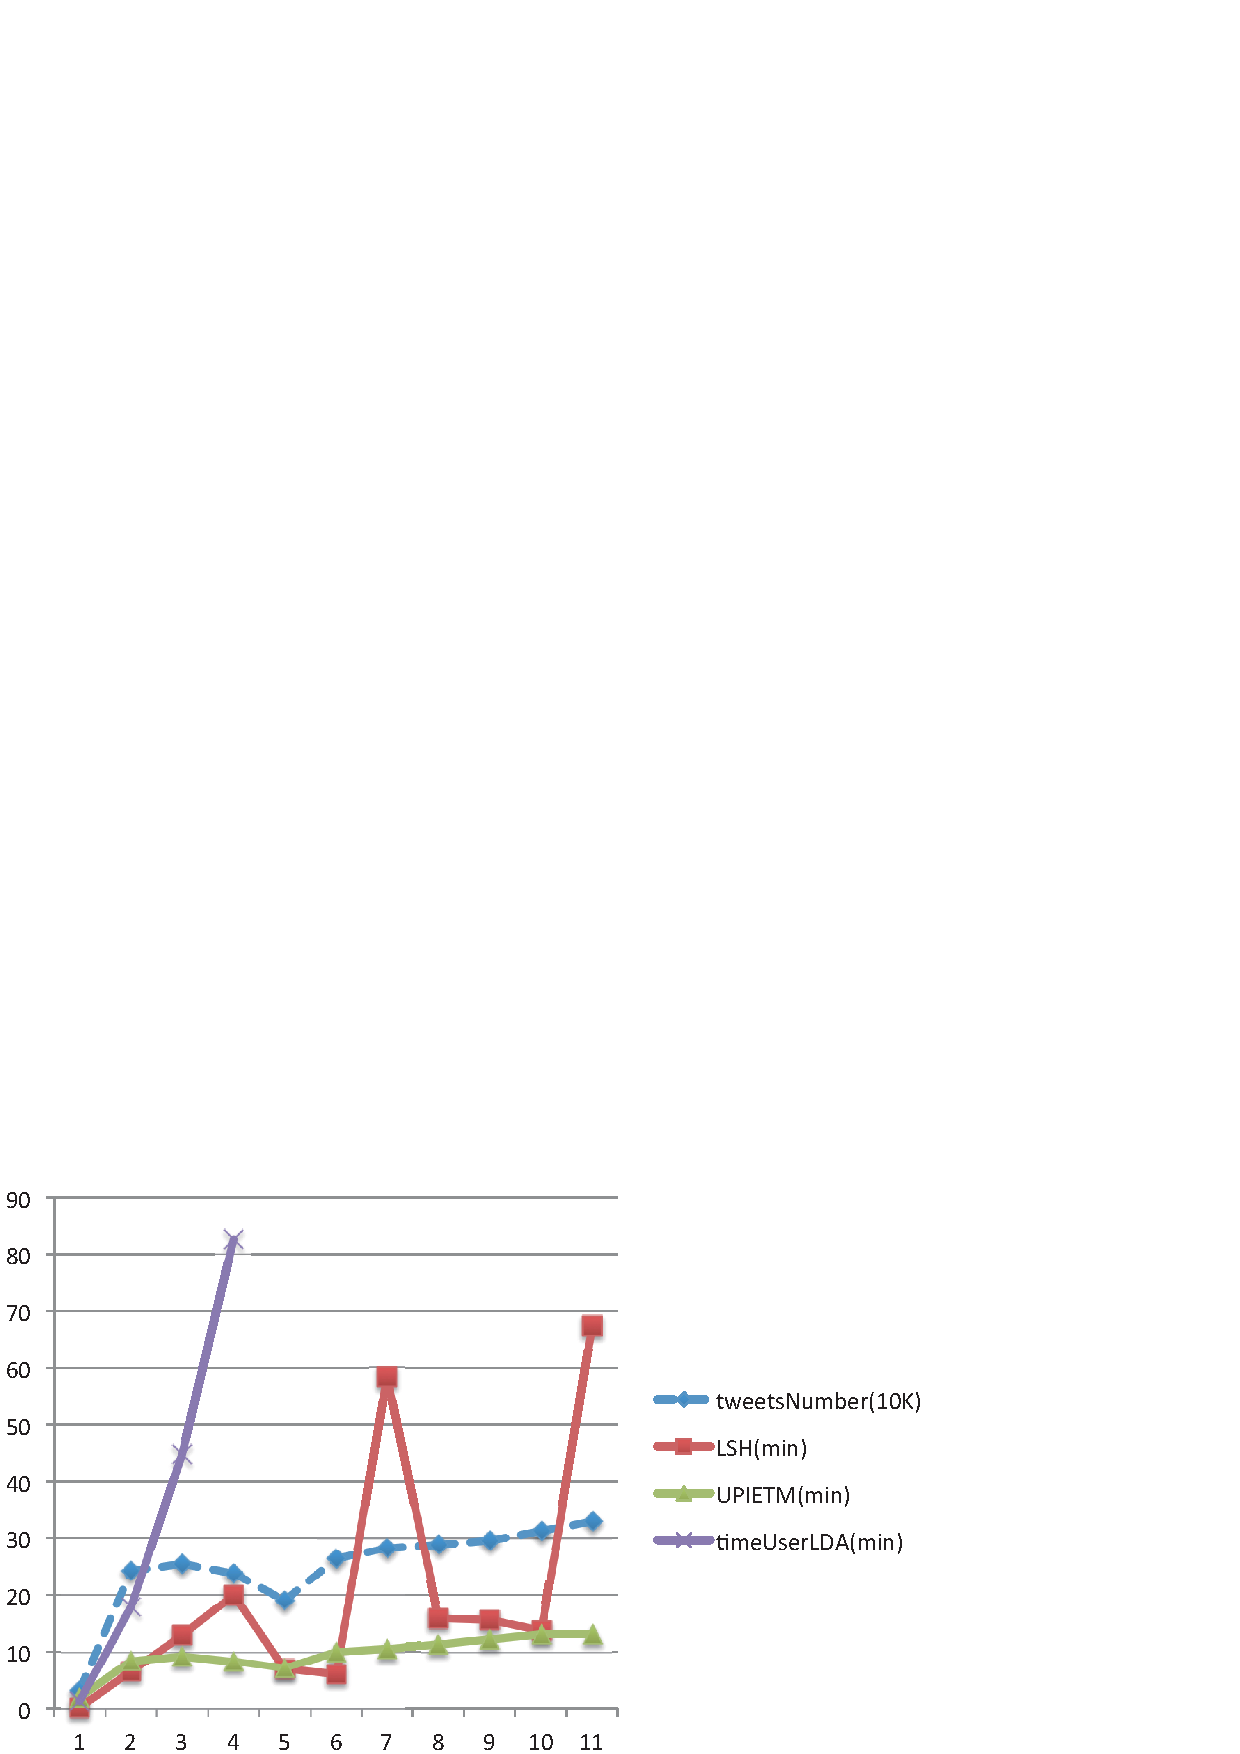
\includegraphics[height=3.1cm]{img/efficiencyCompareWithLSH.pdf}
        }
        \caption{(a) The convergence of complete log likelihood of UMIETM and LDA(with asymmetric priors). The x-axis represents the round of iteration and y-axis shows the complete log likelihood. (b) Efficiency of UMIETM. The x-axis represents the time window, and y-axis shows the duration of processing or the number of tweets in each corresponding time window.}
\end{figure}
\section{Conclusions}
Microblog is mixed with user interests and external events. 
And the external bursty events can be better detected by well user modeling, as the bursty events usually capture the attention from users with different interests.
Since user profile can help to identify user's long term interest, our proposed model UMIETM exploit this vital information into user modeling and event detection.
We further treat the arriving data as stream and run the detection in online learning style.
The experiments demonstrate that our method is effective and efficient for online event detection in microblogs. 
As future work, it would be interesting to discover which groups with specific long term interests are more positive to participate in the discussion of bursty events.

\bibliographystyle{unsrt}
\bibliography{UMIETM}

\end{document}